\section{MTU Discovery}
\label{sec:MTU Discovery}

\subsection{Einleitung}
Mithilfe der \acs{MTU} (Maximum Transmission Unit) wird festgelegt wie gross ein Netzwerkpaket maximal sein darf bevor es in mehrere Pakete aufgeteilt werden muss. Wenn die \acs{MTU} korrekt bestimmt wurde dann kann IP-Paket-Fragmentierung verhindert werden und die Performance der Netzwerkverbindung ist deutlich besser. In einem Netzwerk wird die \acs{MTU} typischerweise pro Netzwerk-Adapter festgelegt. Bei  \acs{IPSec} \acs{VPN} Tunnels kann die \acs{MTU} hingegen pro Tunnel definiert werden auch wenn mehrere Tunnels über den selben Netzwerk-Adapter laufen.
Typischerweise wird die MTU via \acs{PMTUD} (Path MTU Discovery) ermittelt, dabei werden \acs{ICMP} Pakete unterschiedlicher Grösse über die Verbindung gesandt und so kann festgestellt werden welches die maximale Grösse ist die noch ankommt.
Bei \acs{PMTUD} gibt es jedoch ein bedeutendes Problem. Viele Netzwerk-Sicherheits Geräte blockieren ICMP Pakete und so kann die \acs{MTU} der Verbindung nicht korrekt ermittelt werden.
Um die Probleme von \acs{PMTUD} zu umgehen und eine korrekte \acs{MTU} ermitteln zu können haben wir die MTU-Komponente des \tool entwickelt, deren Funktionsweise in den nachfolgenden Abschnitten erläutert wird.

%http://en.wikipedia.org/wiki/Path_MTU_Discovery
\todo{Citation needed}

\subsection{Path MTU Discovery}
Die Path MTU Discovery \acs{PMTUD} ist eine standardisierte Technik um die \acs{MTU} festzustellen.  Bei \acs{IPv4} funktioniert \acs{PMTUD} folgendermassen: Es werden \acs{ICMP} Pakete unterschiedlicher Grösse über die Netzwerkverbindung gesendet. Geräte deren \acs{MTU} kleiner als die Grösse des versendeten Pakets ist verwerfen das Paket und senden stattdessen eine \acs{ICMP} Nachricht mit dem Inhalt "Fragmentation Needed" zurück. So weiss der \acs{PMTUD} Algorithmus dass die versendeten Pakete noch zu gross sind um ihr Ziel zu erreichen. Die versendeten Pakete werden also verkleinert, und der Prozess wiederholt, bis eine Übertragungsgrösse gefunden wird mit der ein Paket den ganzen Pfad ohne Fragmentierung traversieren kann.

Doch wie bereits in der Einleitung angesprochen gibt es bei \acs{PMTUD} ein Problem. Viele Netzwerk-Sicherheit Geräte blockieren \acs{ICMP} Nachrichten. Dies beinhaltet die Errors "Fragmentation Needed" des \acs{PMTUD} Algorithmus. 

%http://en.wikipedia.org/wiki/Path_MTU_Discovery
\todo{Citation needed}

\subsection{MTU-Bestimmung - Idee}
Um die \acs{MTU} der Verbindung zwischen Alice und Bob fest zu stellen werden Pakete mit einer 

% GFX Trim left bottom right top
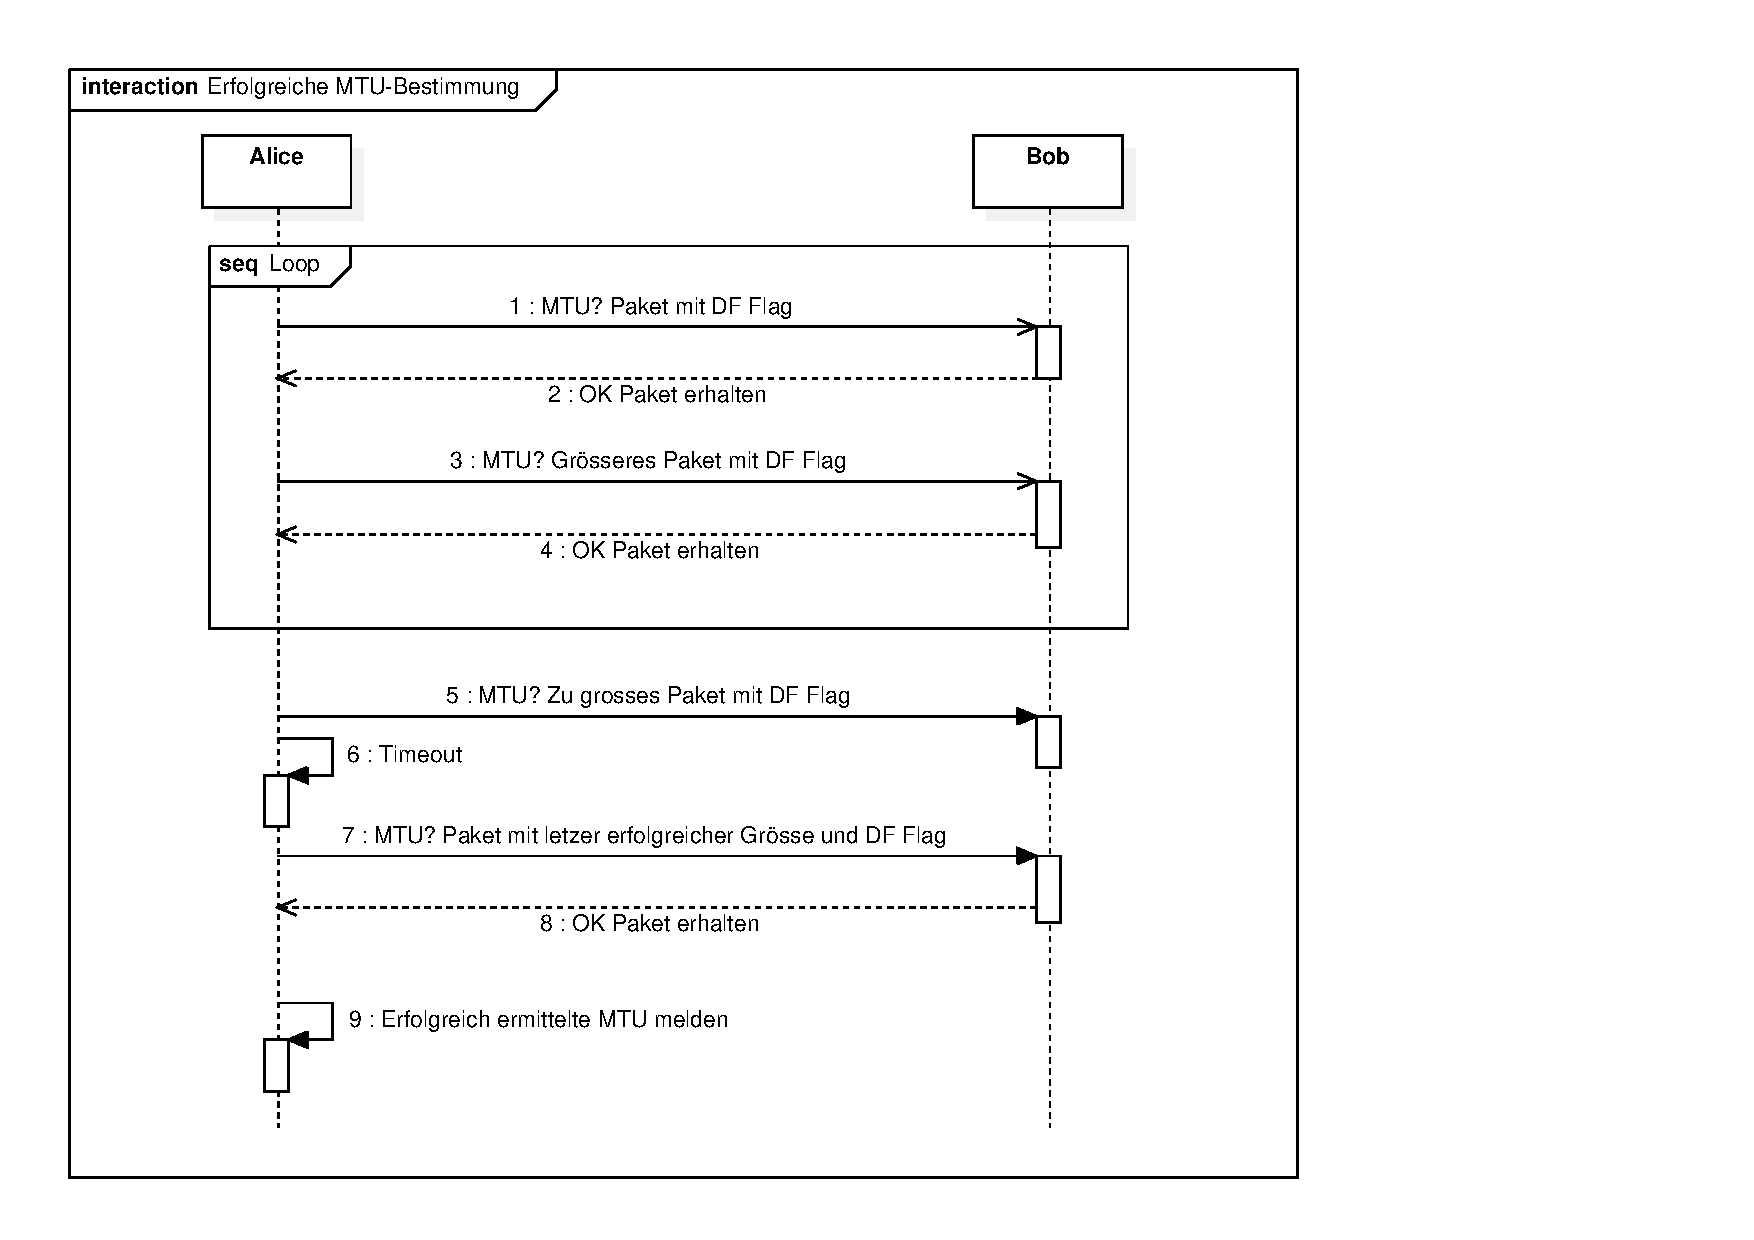
\includegraphics[trim=10 10 200 10,clip,width=\textwidth]{mainpart/implementation/img/MTUBestimmungErfolgreich}

\subsection{MTU-Bestimmung: Fehlerfall}
Dieses Sequenz-Diagramm stellt einen möglichen Fehlerfall bei der Bestimmung der MTU dar. Es zeigt wie das \tool den Fehlerfall behandelt. Alice versucht wie beim erfolgreichen Fall durch das versenden von immer grösseren Paketen die ideale MTU für die Verbindung mit Bob zu finden. Bei Punkt 5 sendet Bob keine Antwort mehr. Alice sendet Bob daher ein Paket mit der letzten erfolgreichen Grösse. Auch auf dieses Paket erhält Alice keine Antwort.  ..todo Grafik anpassen..
Schlussendliche meldet Alice die letzte erfolgreiche MTU mit einer Fehler-Nachricht und bricht den MTU Bestimmungsvorgang ab.

% GFX Trim left bottom right top
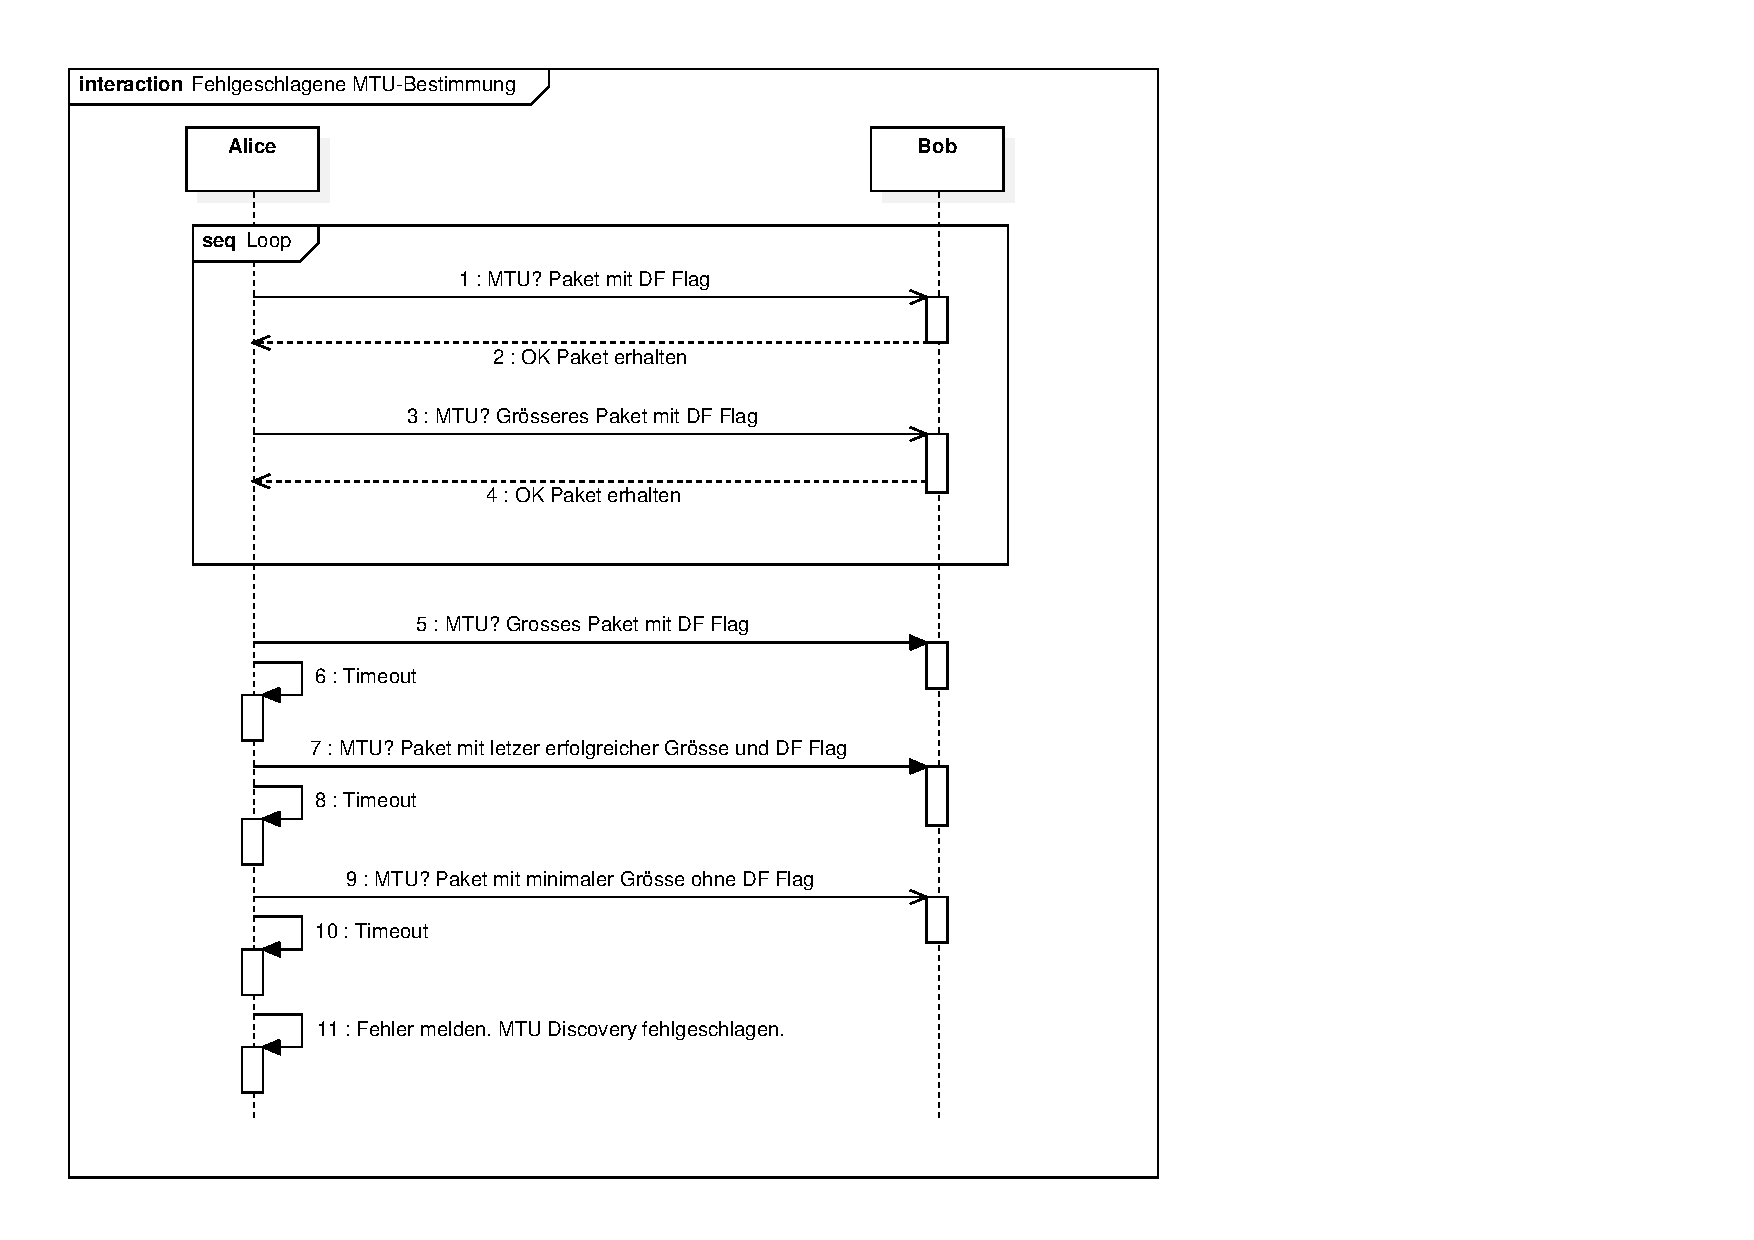
\includegraphics[trim=10 10 265 10,clip,width=\textwidth]{mainpart/implementation/img/MTUBestimmungFehlerfall}